\section{Extension CHORD}
\label{sec:extension_chord}

\subsection{Candidate Site Selection}

Angular resolution of an interferometer is determined by the maximum baseline, which is the distance between the two furthest dishes. CHORD plans to include very long baselines by adding outrigger stations 3300 km and 1000 km away at Green Bank Observatory and Hat Creek Radio Observatory respectively. These outriggers are designed to provide precise localization of bright transient events like Fast Radio Bursts but can't be used for high sensitivity surveys like RRL surveys which require continuous integration over weeks to months. Instead, 16 to 32 additional dishes can be added to the DRAO site, which will feed directly into the main correlator. The purpose of these additional dishes, dubbed Extension CHORD, is to improve the angular resolution of the synthesized beam. The impact on sensitivity will be minimal, as increasing from 512 dishes to 544 dishes only improves the sensitivity by 6 percent, and so it is ignored in the sensitivity analysis of section \ref{sec:sensitivity}.\\

Locations to model extension CHORD were selected by identifying areas of the site that could be developed with minimal effort, such as places that already have disturbed ground and pre-existing power connections. A map of the site showing the proposed labeled locations is shown in Figure \ref{fig:ext_chord_site_map}. For each candidate location we assume 16 additional dishes could be added, with the exception of location G, which is only large enough for 8 additional dishes.

\begin{figure}
	\centering
	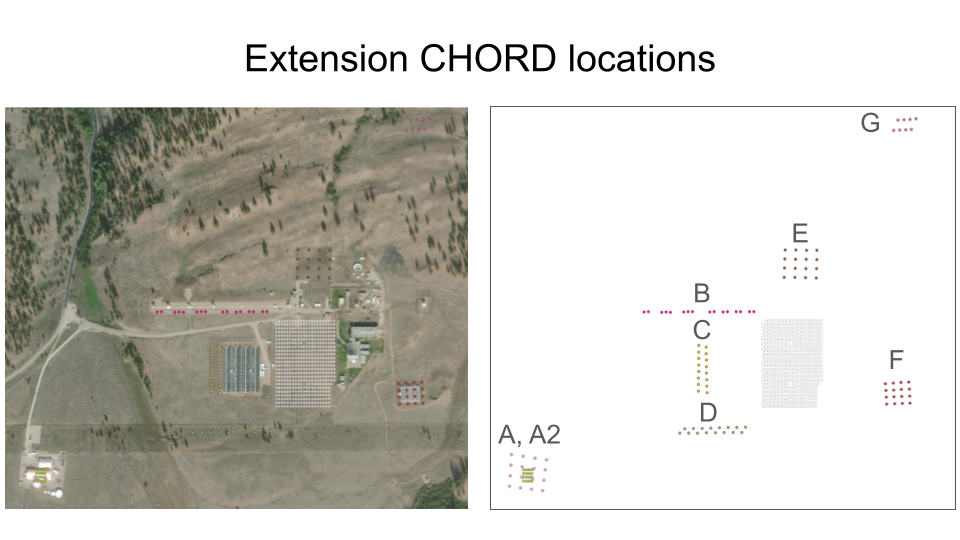
\includegraphics[width=1\linewidth]{plots/ext_chord/site_map.png}
	\caption{Site map for Extension CHORD. Each potential location is labeled A through G. The locations are selected to minimize construction effort by utilizing areas of disturbed ground and pre-existing power connections.}
	\label{fig:ext_chord_site_map}
\end{figure}

\subsection{UV coverage and Synthesised Beam}
The Fourier transform of an image decomposes the image into a sum of spatial sinusoids of different frequencies. Spatial frequencies pointing East-West in the image are labeled $u$, while spatial frequencies pointing North-South are labeled $v$. Each baseline (the vector separating two dishes) of an interferometer is sensitive to a specific spatial frequency, set by the distances $b_{EW}$ and $b_{NS}$ between the two dishes and the wavelength of observation $\lambda$, as given by the equations
\begin{equation}
    u = \frac{b_{EW}}{\lambda}, v = \frac{b_{NS}}{\lambda}.
\end{equation}
Shorter baselines are sensitive to large-scale spatial structures on the sky, while longer baselines provide fine details. The collection of all $u$ and $v$ values sampled is called the UV coverage. The synthesised beam, sometimes called the `dirty beam', is the shape on the sky that a telescope is sensitive to given its UV coverage. To perfectly reconstruct an image of the sky, every spatial frequency would need to be measured. An infinitely sampled UV coverage would produce a delta function synthesised beam, meaning a single point on the sky could be perfectly measured. In practice there are a finite number of baselines, creating a finite UV coverage, so the reconstructed image will contain distortions. The shape of the synthesised beam determines the type of distortions and the overall angular resolution.\\

The UV coverage and synthesised beam for the core CHORD array without any proposed extension dishes are shown in figure \ref{fig:ext_chord_uv_coverage}. The UV coverage is extremely evenly sampled, which is reflected in the Gaussian shape of the synthesised beam. Angular resolution is defined as the Full Width Half Maximum (FWHM) of the synthesised beam and is plotted as a red contour. The angular resolution matches the theoretical values of 7.41' and 5.05' in E-W and N-S respectively, with the asymmetry due to the longer baselines in $v$ as seen in the UV coverage plot.

\begin{figure}
	\centering
	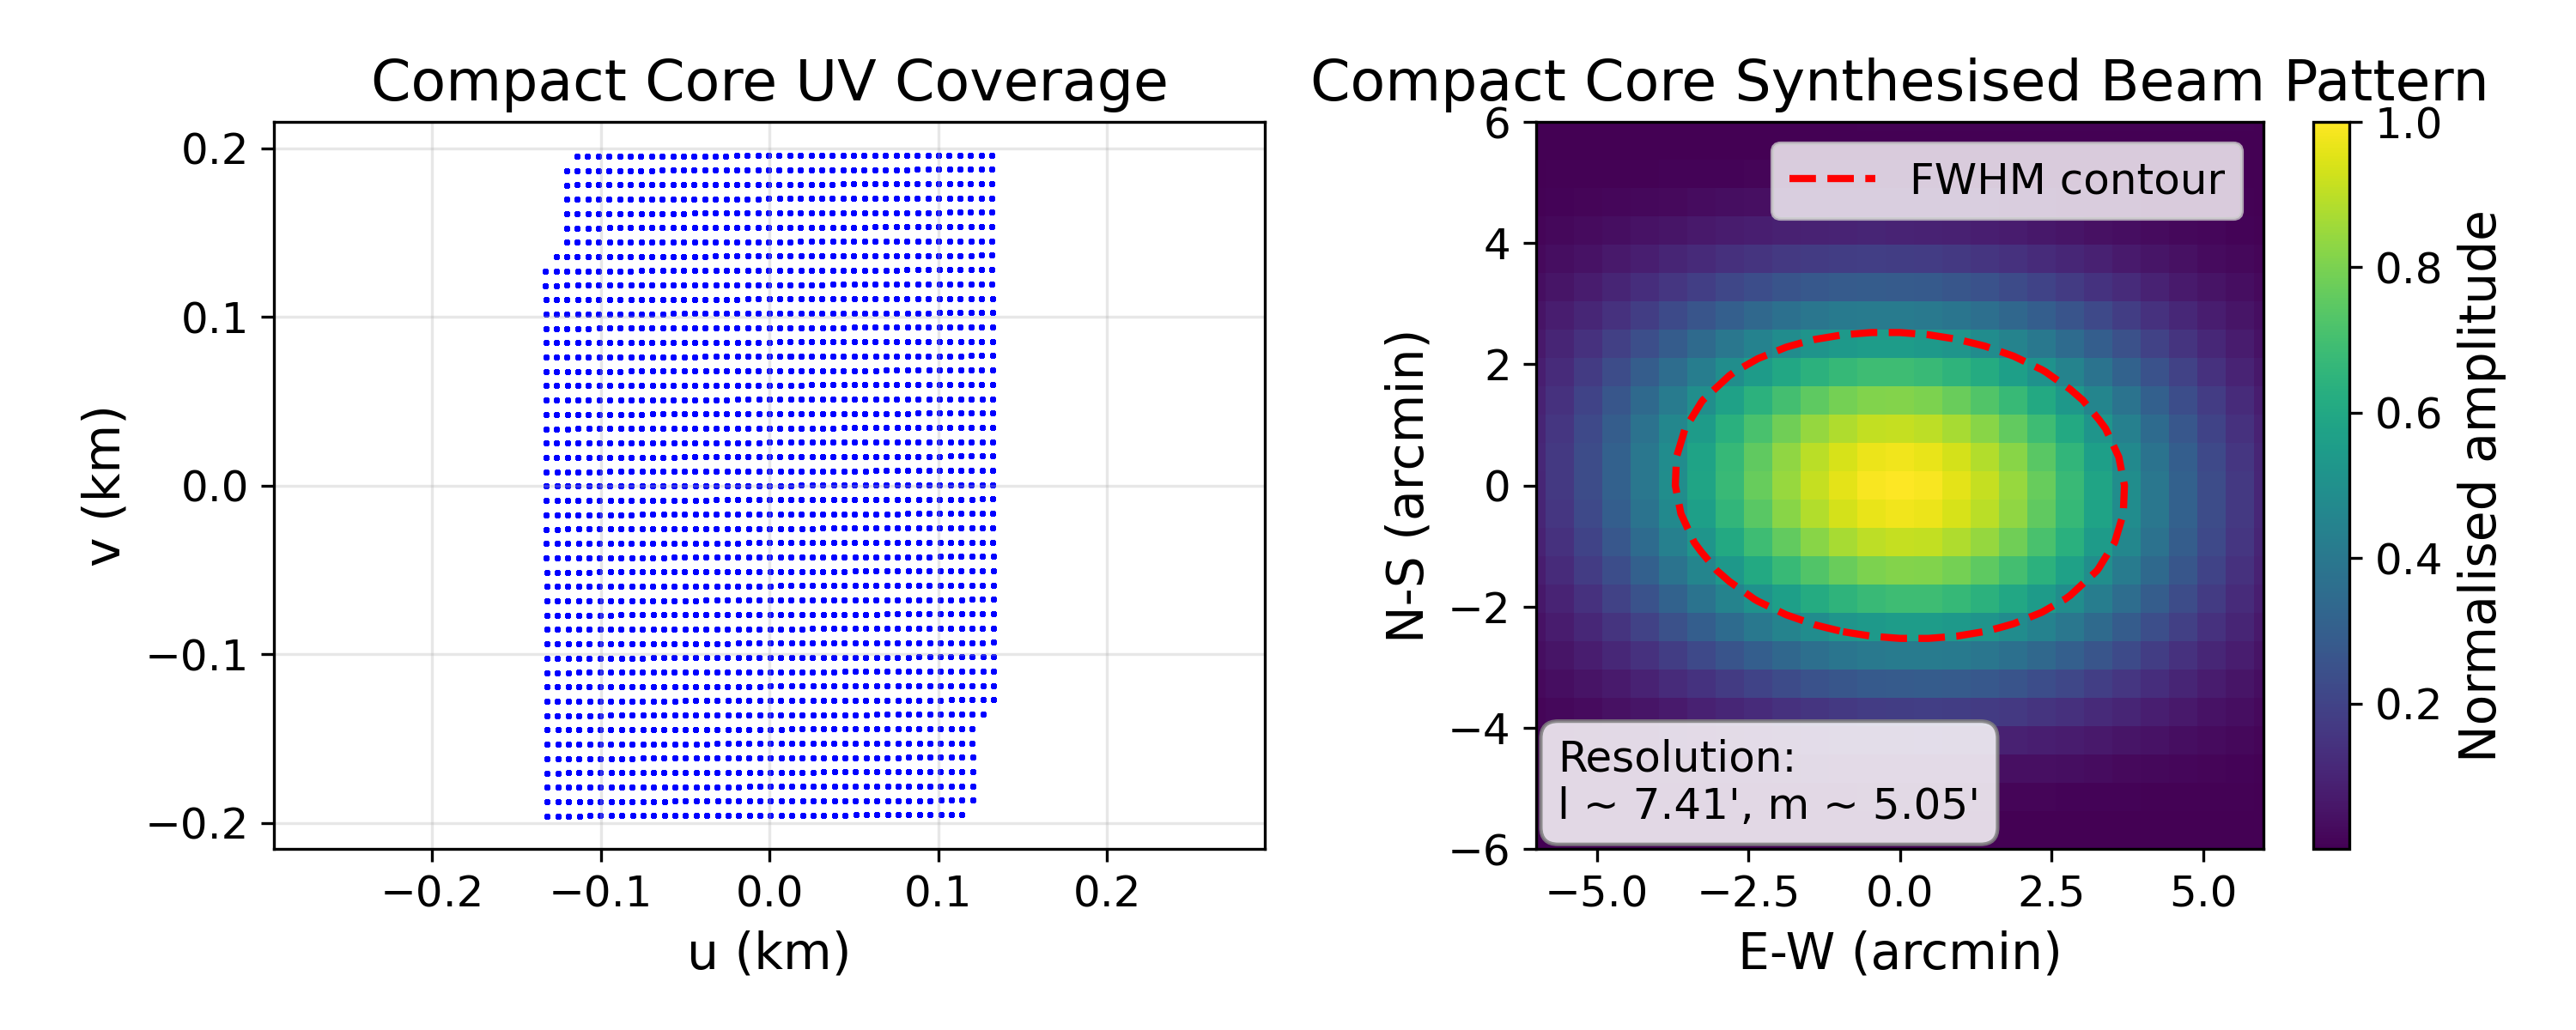
\includegraphics[width=1\linewidth]{plots/ext_chord/uv_coverage_and_beam.png}
	\caption{UV coverage and synthesised beam for the core CHORD array at 900 MHz. The angular resolution is plotted as a red contour of the Full Width Half Maximum (FWHM) of the synthesised beam.}
	\label{fig:ext_chord_uv_coverage}
\end{figure}

\subsection{Weighting Methods}
During imaging the UV plane is discretely sampled by dividing the plane into a grid of cells and summing the contributions from each baseline within a cell. Sensitivity is maximized by weighting each cell equally, which is called natural weighting. However, spatial resolution can be improved by applying more weight to the longer baseline cells, which is called uniform weighting. A middle ground between the two is called robust weighting \cite{briggsHighFidelityDeconvolution1995}, which applies a tunable weight to balance sensitivity and resolution. The weight value $w_k$ for cell $k$ given a robust value $R$ is
\begin{equation}
    w_k = \frac{1}{1 + W_k\, f^2},
    \qquad
    f^2 = \left(5 \cdot 10^{-R}\right)^2 \frac{\sum_k W_k}{\sum_k W_k^2},
    \label{eq:briggs}
\end{equation}
where $W_k$ is the number of baselines that fall in cell $k$ and the robust value $R$ takes the suggested range of [-2, +2]. For $R \to +2$ the factor $f^2 \to 0$ and robust weighting approaches natural weighting. For $R \to -2$ the factor $f^2$ becomes large, so $w_k \to 1/(W_k f^2) \propto 1/W_k$, which down-weights densely sampled cells and approaches uniform weighting. Intermediate values of $R$ interpolate smoothly between the two extremes.\\

Improving angular resolution comes at the cost of sensitivity, since signal from densely sampled cells is down-weighted. The amount of sensitivity lost can be quantified by the noise factor, which is the ratio of the sensitivity of the applied weighting to the sensitivity of natural weighting. The noise factor is given by
\begin{equation}
    \text{Noise Factor} = \frac{\sigma_R}{\sigma_\text{nat}} = \frac{\sqrt{\sum_k w_k^2} \big/ \sum_k w_k}{\sqrt{\sum_k W_k^2} \big/ \sum_k W_k}.
    \label{eq:noise_factor}
\end{equation}

\subsection{Evaluating Beam Patterns}
The impact of adding location A to the CHORD array is analysed in detail to illustrate how irregularly sampled UV coverage affects the synthesised beam. The UV coverage in the top left of figure \ref{fig:loc_A_cov_and_beam} shows the added long baselines, which appear as densely sampled zones at $\pm 0.6$ km in $u$ and $\pm 0.3$ km in $v$, while the rest of the plane remains unsampled. The top right plot shows the combined core plus location A beam using natural weighting, where the beam is almost unchanged compared to the core array alone shown in figure \ref{fig:ext_chord_uv_coverage}. This is expected since adding only 16 dishes has a minimal impact compared to the 512 dish core array. The bottom left plot shows the beam using uniform weighting, which applies more weight to location A than to the core. The uniform beam has multiple peaks, which arise from the UV plane being poorly sampled. While the central peak does achieve an angular resolution close to the theoretical resolution of $1.69'$ and $3.13'$ in E-W and N-S respectively, the multiple peaks make it impossible to apply this angular resolution to practical observations. Instead, we define the `effective angular resolution' as the maximum extent of the FWHM contours in E-W and N-S, plotted as an ellipse. Based on the effective angular resolution, the uniform beam achieves $4.92'$ and $3.91'$ in E-W and N-S respectively, at a noise factor cost of 2.83. To understand the trade-off between angular improvement and sensitivity loss, the bottom right plot shows effective resolution versus noise factor for a range of robust values, where a noise factor of exactly 1 corresponds to natural weighting and the maximum noise factor corresponds to uniform weighting. From the elbow curve we can see that a roughly 25\% improvement in angular resolution can be achieved for a marginal increase in noise factor.

\begin{figure}
	\centering
	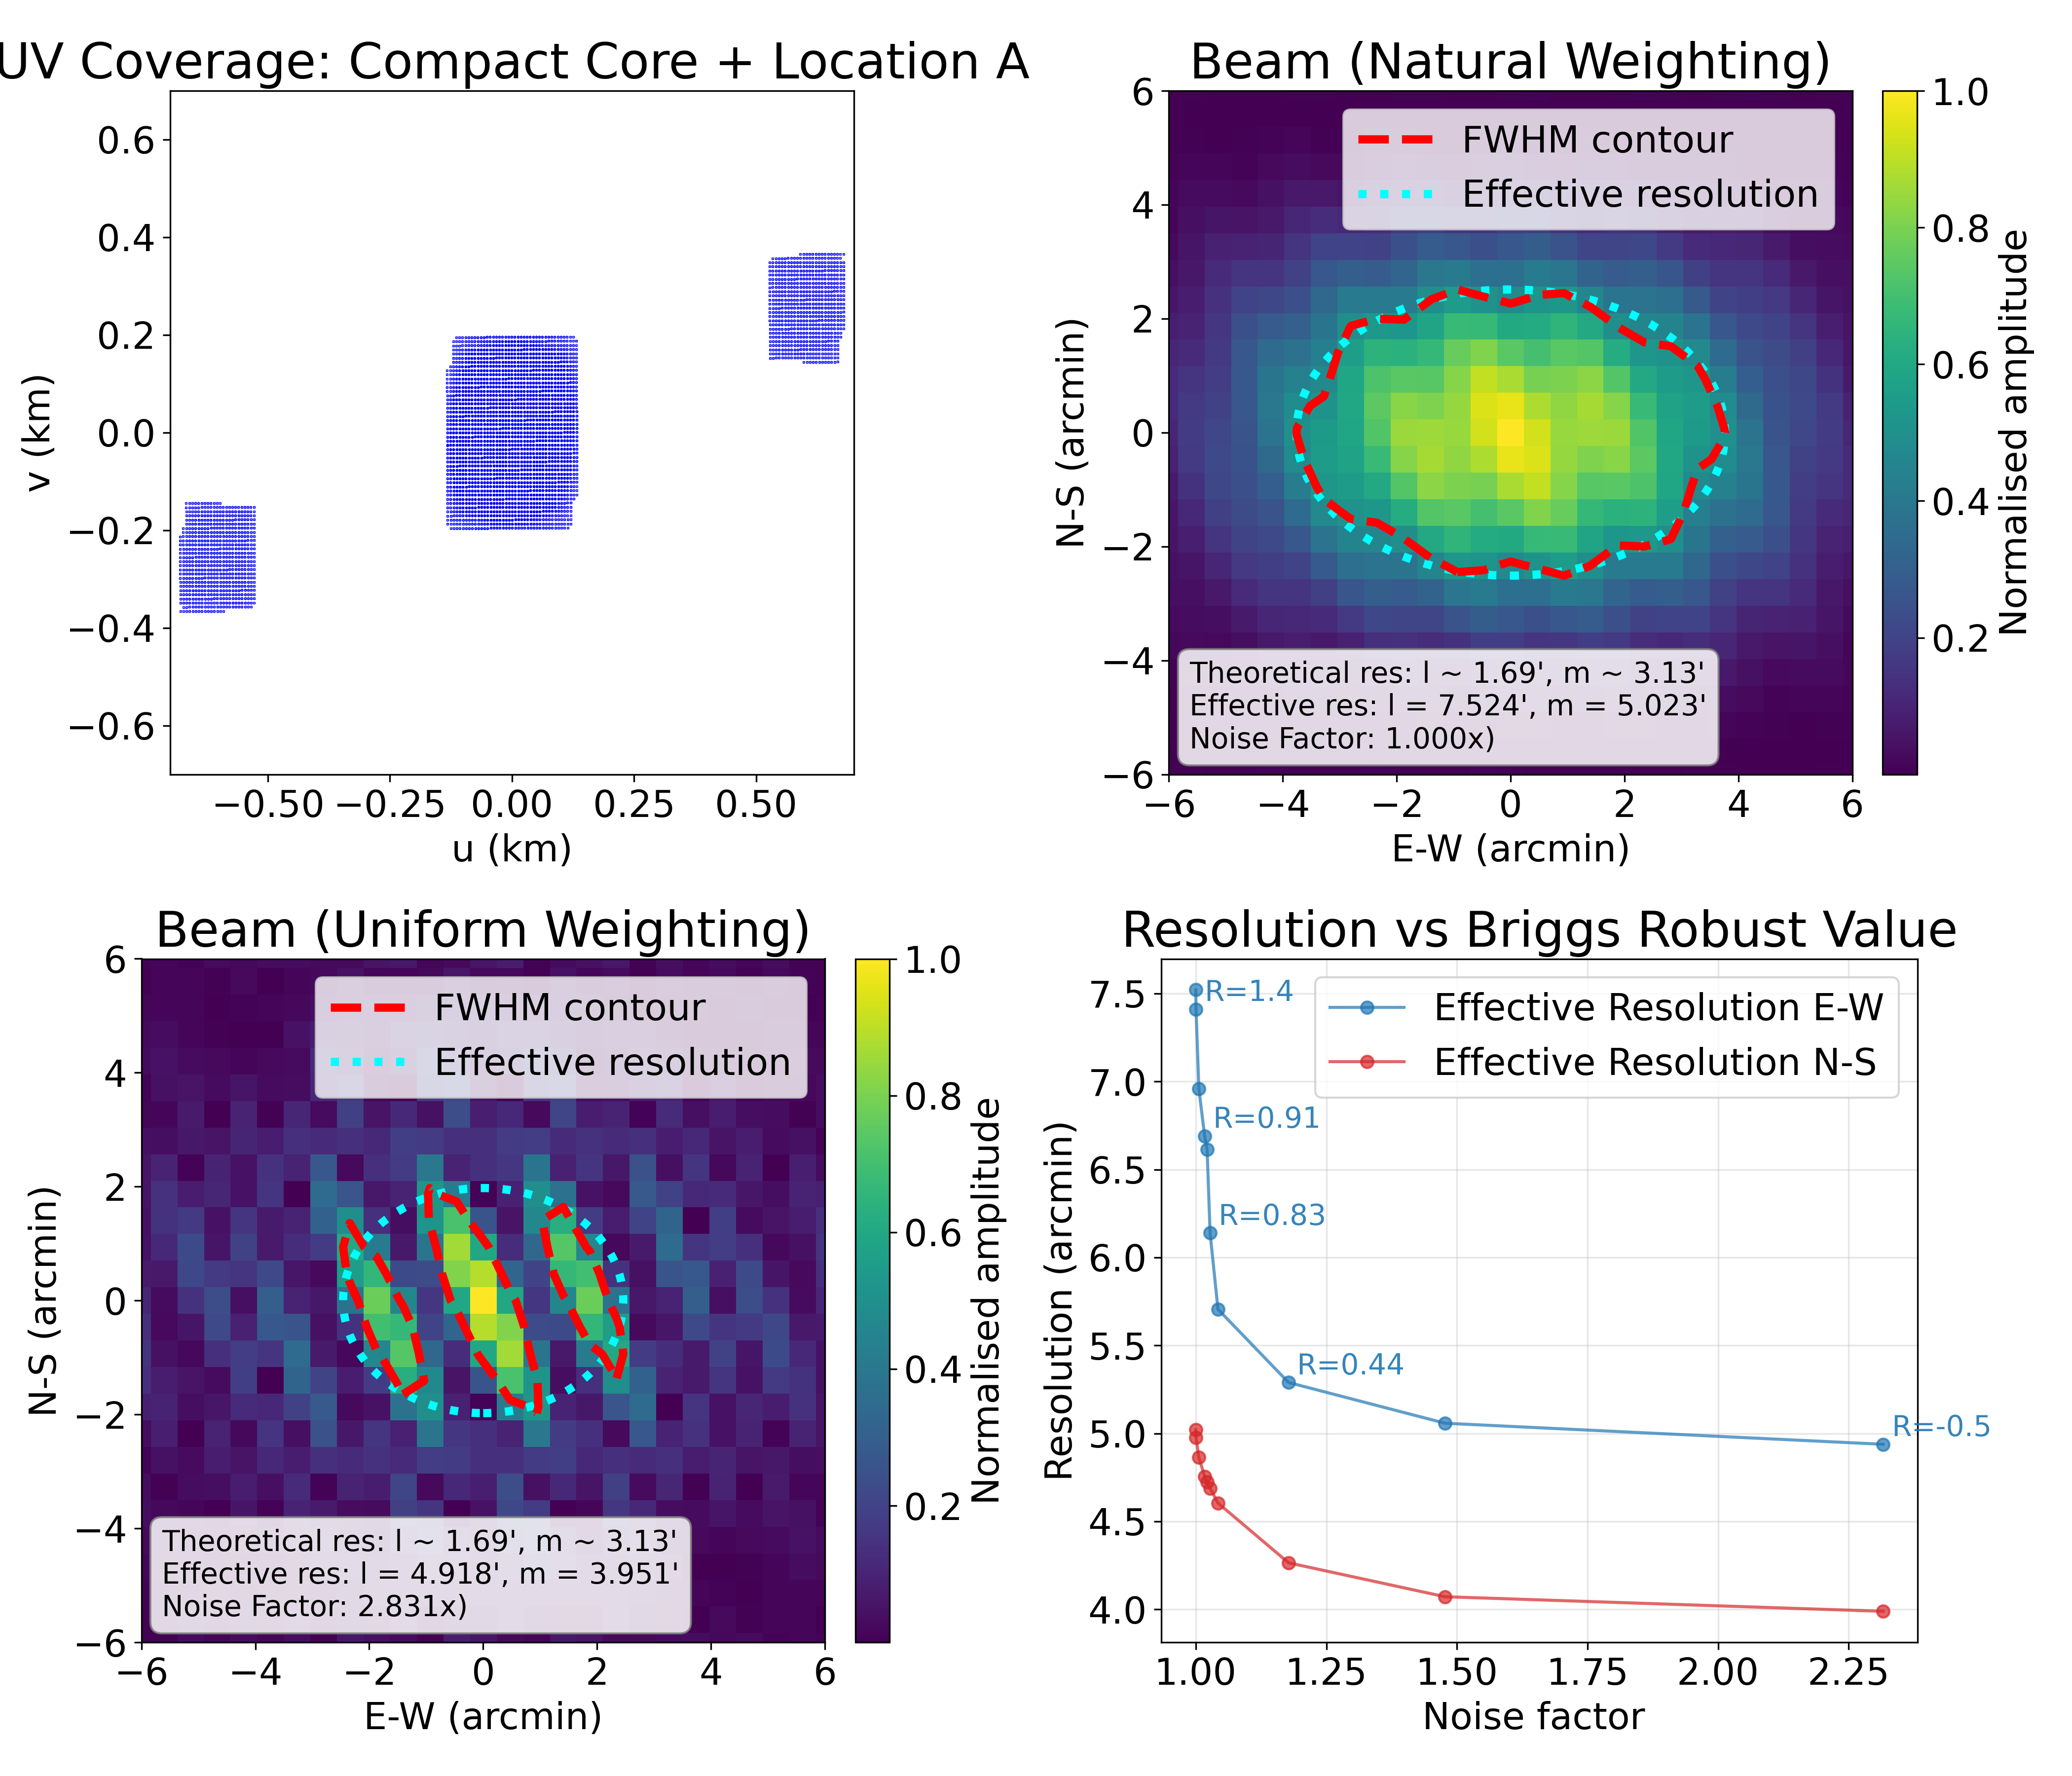
\includegraphics[width=1\linewidth]{plots/ext_chord/loc_A_cov_and_beam.png}
	\caption{Effect of adding location A to the core CHORD array. Top left: UV coverage. Top right: synthesised beam under natural weighting. Bottom left: synthesised beam under uniform weighting, with the effective angular resolution plotted as an ellipse. Bottom right: effective resolution versus noise factor over a range of robust values.}
	\label{fig:loc_A_cov_and_beam}
\end{figure}

